\documentclass[a5paper,twoside]{scrbook}
\usepackage[ngerman]{babel}
%Schrift Quattrocento
\usepackage{quattrocento}
\usepackage[T1]{fontenc}
%Schweizer Anführungszeichen
\usepackage[german=swiss]{csquotes}
%Erlaubt Einsatz von Farbe
\usepackage{color}
%UTF 8
\usepackage[utf8]{inputenc}
%Ermöglicht Zierkapitälchen zum Anbsatzanfang
\usepackage{lettrine}
%Fourier Ornamente für Seitenkopf
\usepackage{fourier-orns}
%Ums Seitenkopf zu manipulieren
\usepackage{scrpage2} 
\pagestyle{scrheadings} 
%Auf jeder Seite ausser Kapitelanfängen oben Linie mit zwei Zeichen in der Mitte
\chead{\color{red}\hrulefill\hspace{0.2cm} \floweroneleft\floweroneright \hspace{0.2cm} \hrulefill}
%Kapitelüberschriften in Schriftart des Deckblatts
\addtokomafont{chapter}{\color{red}\rmfamily\Huge\centering\it}
%Schriftart für grosse Anfangsbuchstaben
\input Zallman.fd
\renewcommand{\LettrineFontHook}{\usefont{U}{Zallman}{xl}{n}}
%Schrift für Überschriften
\def\FontH{\fontsize{10pt}{0mm}\usefont{T1}{frc}{m}{n}}
%Grafiken einbinden
\usepackage{graphicx}
%Für Kapitel Gespenst Jonathan Rahmen ermöglichen
\usepackage{mdframed}
%Definition Rahmen: links dicker roter balken
\mdfdefinestyle{mystyle}{
        %topline=false,
        bottomline=false,
        rightline=false,
        linewidth=2pt,
        linecolor =red}
%Abstand zw. Wörtern darf zwecks Blocksatzbildung in Ausnahmefällen bis 1em breit werden.
\setlength{\emergencystretch}{1em}
%bessere Mikrotypographie (margin kerning insb. am Rand)
\usepackage{microtype}
%Seitenzahlen fett
\addtokomafont{pagenumber}{\bfseries}
%To-Do Kommentare einfügen -> \todo{} \missingfigure{}
\usepackage{todonotes}
% used for the 'logo'
\usepackage{tikz}            


%%%%%%%%%%%%%%%%%%%%%%%%%%%%%%%%%%%%%%%%%%%%%%%%%%%%%%%%%%%%%%%%%%%%%%%%%%%%%%%%%%%%%%%%%%%%%%%%%%%%%%
\begin{document}
%titelseite
\begin{titlepage}
	\begin{center}
		\vspace*{3\baselineskip}
		\FontH{\Huge \color{red} Geschichten für\\ meine Töchter}\\ 
	\end{center}
		\vspace*{4\baselineskip}
	
	\begin{center}
		\begin{tabular}{p{7cm}p{5cm}}
			\textbf{\large \color{red} Gordon Wiegand} & \textbf{\large \color{red}  Linda Wiegand}\\
			\textbf{\large \color{red}\it Texte} & \textbf{\large \color{red}\it Illustrationen}\\
		\end{tabular}

	\end{center}
		\vspace*{4\baselineskip}
	\begin{center}
		% create logo (letter H within a circle)
		\begin{tikzpicture}
   			\node[circle,draw,ultra thick,red] at (0,0) {{\large$\mathcal{GL}$}};
		\end{tikzpicture}
		% logo titl
	\end{center}

\end{titlepage}
%Bild Seite 2
\begin{figure}[ht]
\centering
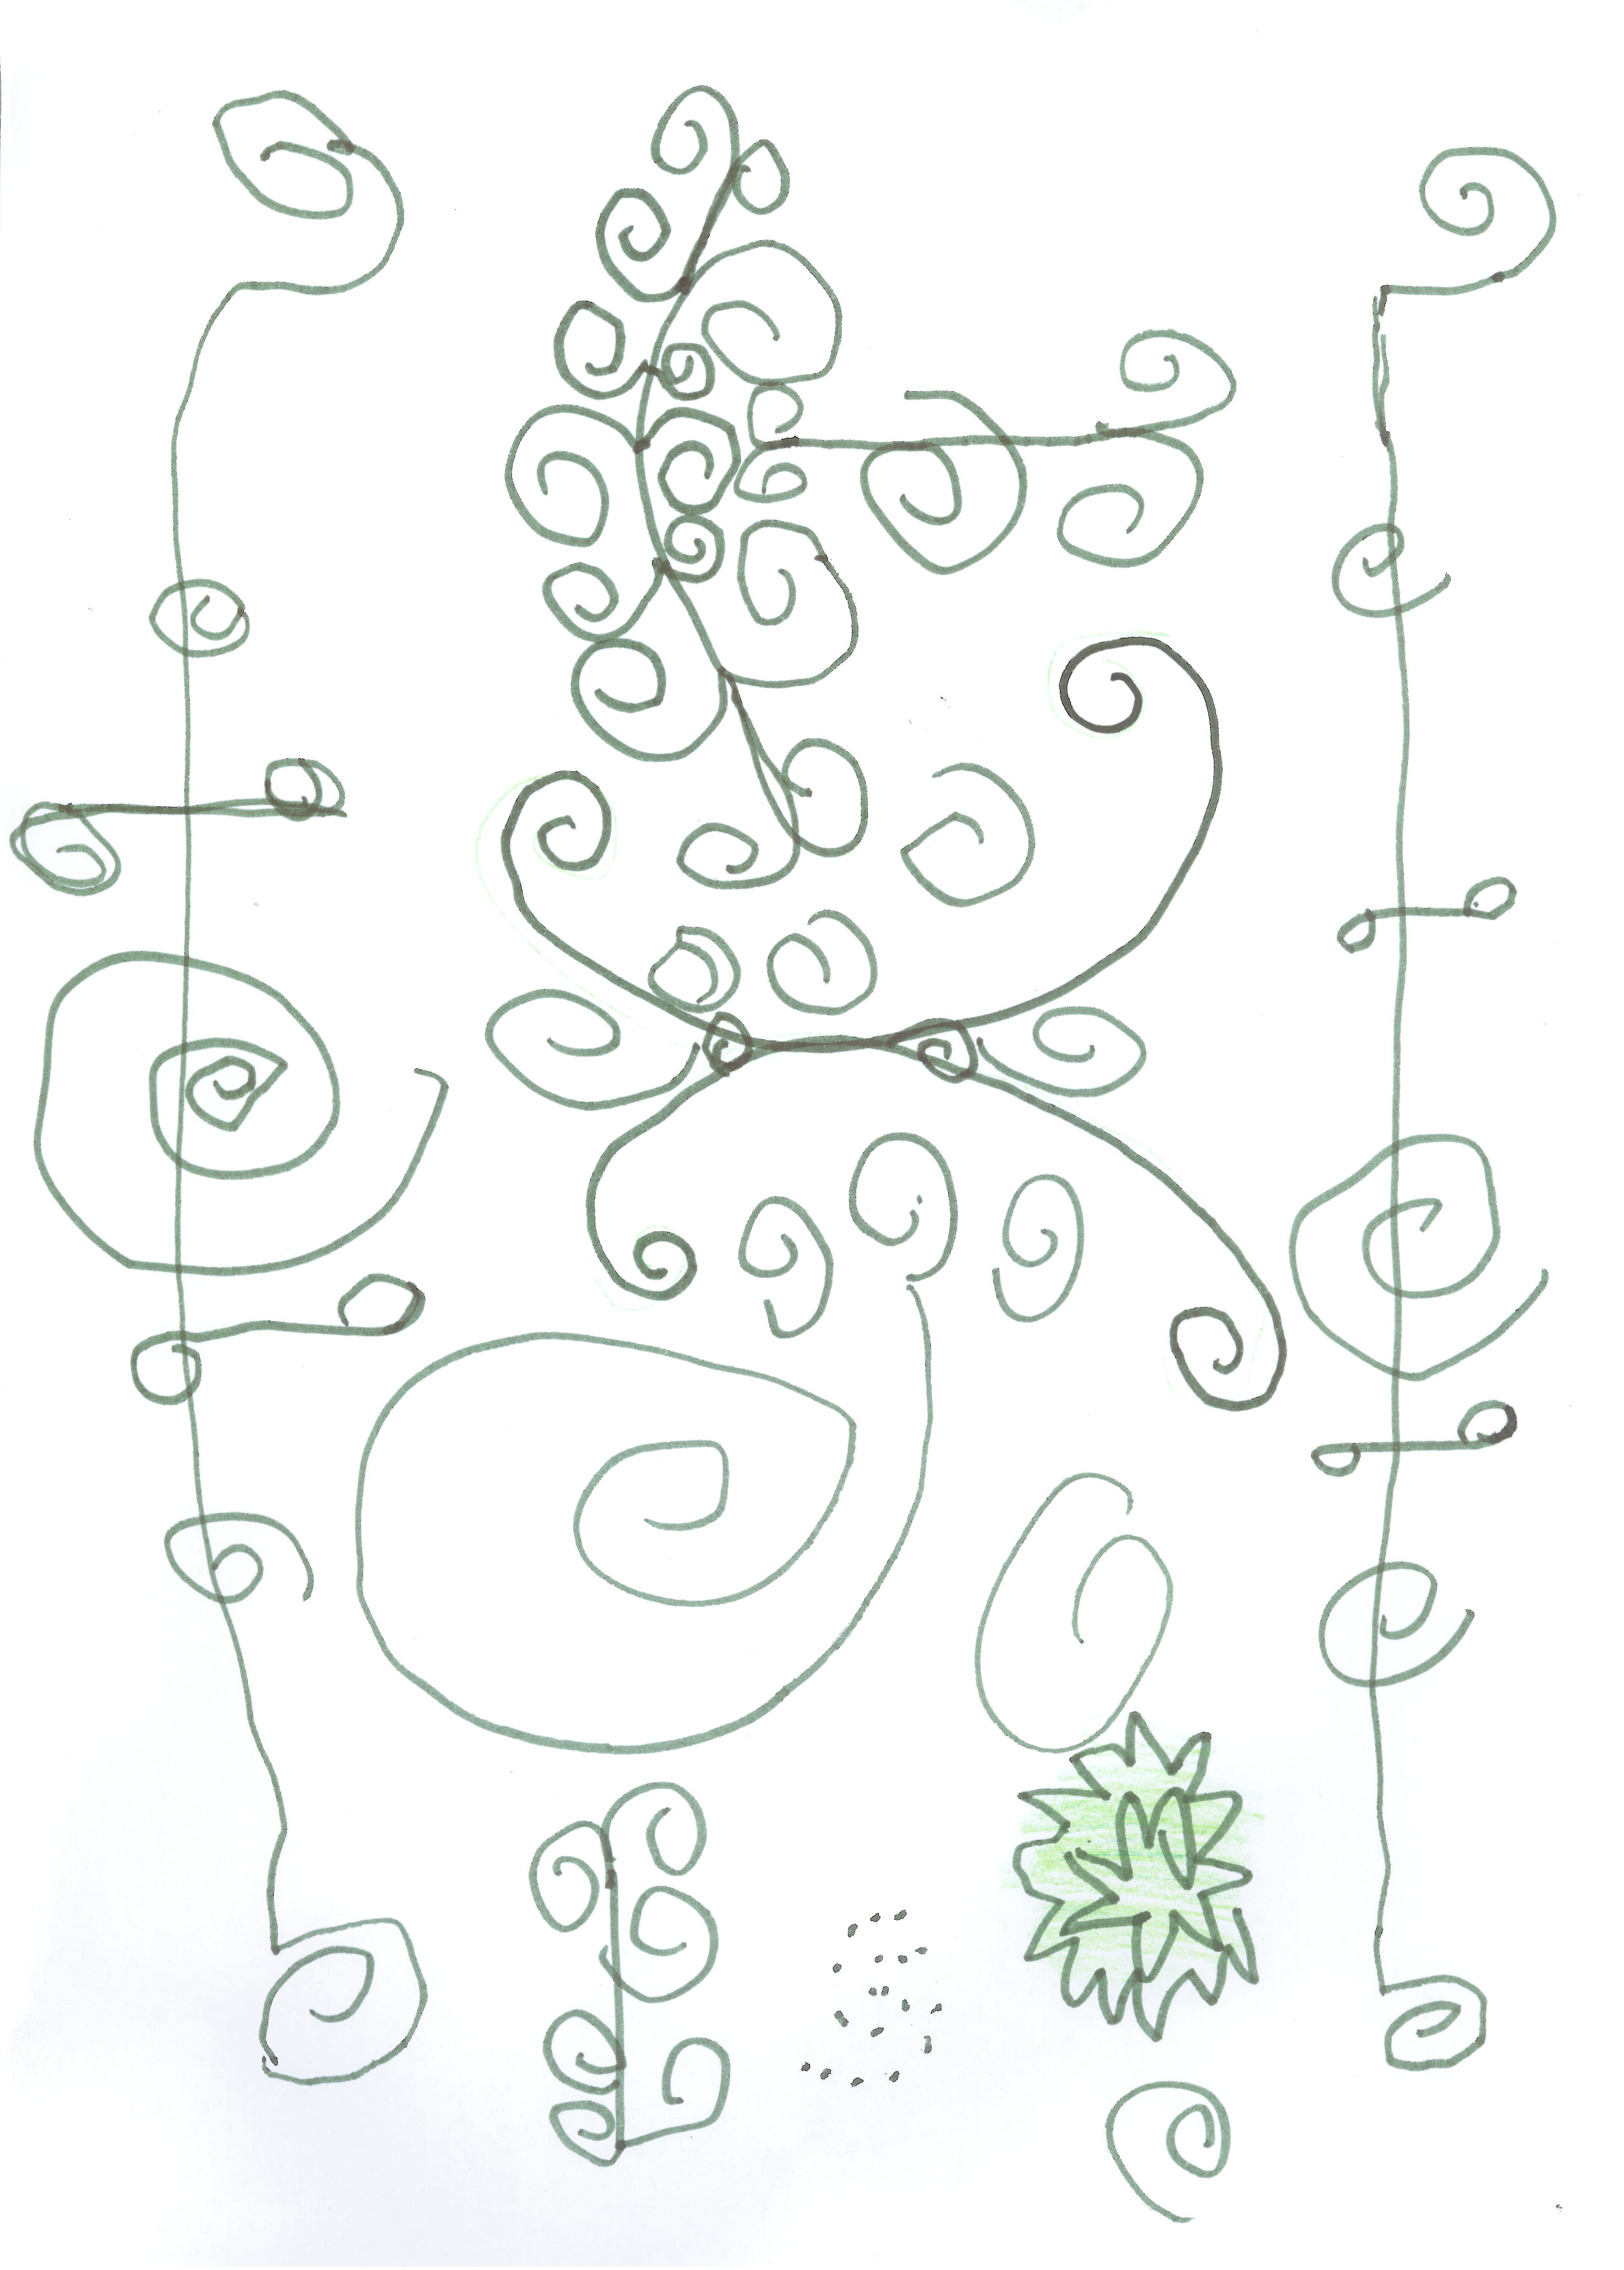
\includegraphics[width=\textwidth]{bilder/titel.jpg}
\end{figure}
%Kapitel einfügen
\chapter*{\FontH{\Huge Pinarella}}
\addcontentsline{toc}{chapter}{Pinarella}
\lettrine[lines=2]{\color{red}P}{}inarella war ein Schmetterling. Träge lag sie wie jeden Morgen auf dem Regal im Wohnzimmer der Familie Emil und liess sich die Sonne auf die Flügel scheinen. Sie gähnte so laut das Schmetterlingsdamen eben können und blickte sich gelangweilt im Zimmer um. Pinarella war nämlich kein einfacher Schmetterling, nein, sie bestand aus einem Körper aus Holz und die Flügel waren aus bunter Folie gemacht. Schön sah das zwar aus, aber zum Fliegen taugte so ein Körper nicht. Cornelia, die Tochter der Emils hatte Pinarella gebastelt, als sie so ungefähr in der dritten Klasse gewesen war. Aber das ist jetzt schon viele Jahre her, Cornelia hatte selbst schon zwei Kinder und mit denen war sie gerade zu Besuch bei ihren Eltern. Eigentlich wohnte Pinarella gar nicht auf dem Regal, sondern hing für gewöhnlich an einer Schnur über dem Ofen. Aber das letzte Mal als Cornelia mit den Enkelinnen dagewesen war, ist sie beim Spielen auf dem Boden gelandet und von da hat sie jeman auf das Regal gelegt. Bisher hatte sich noch niemand die Mühe gemacht, sie wieder aufzuhängen, aber das war Pinarella egal. Beide Orte sind genau gleich langweilig, so viel war klar. Deswegen war es auch ganz gleichgültig, wo sie gelagert wurde.


Spielen konnte sie allerdings auch bei den Emils. Besonders Jette, die jüngste Tochter von Cornelia machte das sehr gerne.  Jette war allerdings noch zu jung, um die Schönheit Pinarellas zu verstehen. Sonst würden sie wahrscheinlich nicht gar so garstig und nachlässig mit ihr umgehen. Mal wurde sie an den Flügeln gezogen, die dann umständlich von Frau Emil wieder festgeleimt werden mussten, dann wurde sie unachtsam unter einem Berg Legosteine vergraben. Und einmal wurde sie sogar mit auf die Pergola genommen und dann dort vergessen. Die ganze Nacht fror Pinarella ganz fürchtlerlich.

Jette war allerdings ein liebes Kind, das wusste Pinarella, deswegen nahm sie ihr das alles auch nicht übel. Sie war einfach noch zu jung. So viel wusste Pinarella über die Menschen: wenn sie klein sind, überlegen sie manchmal nicht, was so alles passieren kann, wenn sie dies und jenes machen. Gerade gestern ist Jette in alleine in ihr Stühlchen geklettert und dabei sehr unsanft abgestürzt. Das war ein Weinen! Und Jette hatte sich selbst bestimmt nicht mit Absicht weh getan, hatte Pinarella überlegt und so ging es wohl auch mit ihr, wenn Jette ihr mal wieder einen Fühler abgebissen hatte.

Auf dem Regal war Pinarella jetzt zwar sicher vor Jette, aber eben auch alleine. Jette war viel zu klein, um sie so weit hoch zu kommen. Lieber wieder einen Flügel verlieren, dachte Pinarella, als den ganzen Tag hier zu liegen. 

\enquote{Schade} seufzte Pinarella, \enquote{wirklich schade, dass ich kein richtiger Schmetterling bin. Es ist ja schon lustig, mit Jette zu spielen, aber die ist einfach so selten zu Besuch. In der Zwischenzeit ist es doch immer sehr langweilig. Da wäre es ja doch viel lustiger, wenn ich hinaus fliegen könnte in die Welt, um mit anderen Schmetterlingen zu spielen.} 

An diesem Morgen war Jette mal wieder sehr früh munter geworden. Cornelia, die Jette selbstverständlich nur \enquote{Mama}  nannte und sie waren im Wohnzimmer und Cornelia war wieder eingeschlafen. Pinarella hatte das gar nicht gemerkt. Jette sass auf dem Boden und versuchte vergeblich ihrem Püppchen die Hosen anzuziehen. Wenn man erst zwei Jahre alt ist, klappt so etwas manchmal noch nicht so gut und ausserdem waren es sowieso Hosen für eine viel kleinere Puppe. Die Sache klemmte und damit auch die Lust von Jette, weiter mit der Puppe zu spielen. Gerade als sie sich umsah, um zu sehen, womit man als nächstes so spielen könnte, hörte sie die Klage von Pinarella. 

\enquote{Was ist denn mit dir los?} fragte Jette. Pinarella war verwirrt. Schon oft hatte sie versucht mit Menschen zu reden, aber so laut sie auch geschrieen hatte, nie hat sie jemand gehört.

\enquote{Kannst Du mich verstehen?} fragte sie daher ganz ungläubig. 

Jette nickte bloss. 

\enquote{Mir ist langweilig.} sagte Pinarella, niemand spielt mit mir, meine Flügel sind schon voller Staub.

\enquote{Dann komm doch hier zu mir geflogen!} schlug Jette vor, die den Unterschied zwischen einem echten Schmetterling und einem gebastelten noch nicht so genau kannte. Und obwohl Jette das gar nicht so genau interessierte, erklärte Pinarella ihr den Unterschied. Ihr war das nämlich wichtig. Jette verstand nicht alles, aber eines war klar: Pinarella wollte auch gerne fliegen können, um mit anderen Schmetterlingen spielen zu können. Das verstand Jette sogar gut, sie spielte ja auch am liebsten mit anderen Kindern.

\enquote{Dann helfe ich Dir!} beschloss Jette, hatte aber noch keine Ahnung, wie. Aber das ist normal bei Zweijährigen. Die beschliessen immer Sachen, von denen sie noch nicht wissen, wie man das dann genau macht. Zuerst musst Pinarella mal von dem Regal herunter, das war offensichtlich. Das Regal war schon sehr hoch, sogar noch höher als Papa gross ist, schätzte Jette. Der konnte einen aber hoch nehmen, wenn man die Arme in die Luft streckt, Regale machen so etwas wohl aber nicht. Jette hatte bereits ein bisschen Lebenserfahrung. Und die sagte ihr auch, dass man wohl etwas zu Hilfe nehmen musste.

Die beide sahen sich im Zimmer um, was wohl genau diese Hilfe sein könne. Jette hatte plötzlich eine Idee. Wenn sie mit dem Wasserhahn vom Waschbecken spielen wollte, schob sie sich immer das Schemelchen hin und stieg darauf. Für das Waschbecken war sie nämlich auch noch zu klein.  Aber das Schemlechen war natürlich im Badezimmer und wenn man dort hin wollte, würde Mama bestimmt munter werden. Pinarella und Jette mussten seufzen. Beinahe gleichzeitig sahen sich die beiden an, dann zum Stuhl, dann wieder sich. So leise wie eine Zweijährige eben kann, lief Jette zu dem Stuhl und schob ihn so vorsichtig wie möglich in Richtung Regal.

\enquote{Mach keinen Quatsch!} Mama war von dem Quitschen munter geworden, drehte sich aber zum Glück nochmals auf die Seite und schlief weiter. Jette und Pinarella hatten den Atem angehalten, den Jette mit einem lauten {\it Pffff.} jetzt wieder raus liess. Das war knapp. Wenn Mama gemerkt hätte, was Jette vor hat, wäre sie bestimmt dagegen gewesen. Ganz leise kletterte Jette jetzt auf den Stuhl. Noch immer reichte sie nicht bis oben hin. Zum Glück sah Jette sofort dendem Rückenkratzer vom Opa, den konnte sie nehmen und tatsächlich! Es klappte! Jette kam gerade so bis an das obere Ende des Regals, konnte Pinarella an einem Fühler erwischen und zog sie vom Regal herunter.

Mit einem leisen {\it Plopp} landete Pinarella auf der Couch, aber zum Glück weit genug von Mama entfernt. Jette kletterte vom Stuhl herunter, was gar nicht so einfach war, nahm Pinarella, öffnete das Fenster und mit einem lauten 

\enquote{Jippie, flieg Pinarella!} war Jette den Holzschmetterling aus dem Fenster.

Natürlich konnte Pinarella nicht fliegen. Sie stürzte jäh ab und raste in Richtung Boden. 

\enquote{Da wird bestimmt noch mehr kaputt gehen, als nur ein Fühler.} dachte Pinarella. Gerade in dem Moment ging die Sonne hinter den Bergen auf. Und genau als Pinarella in der Luft war, traf sie der allererste Sonnenstrahl des Tages. Pinarella konnte ihn auf ihren Flügeln spüren und instinktiv zuckte sie zusammen und da geschah es. Ihre Flügel bewegten sich! Erst langsam, dann immer schneller und noch bevor Pinarella auf dem Boden aufschlagen konnte, flog sie. Aus der Spielzeugpinarella war ein richtiger Schmetterling geworden. Höher und immer höher flog sie, fast so hoch wie das Haus und wieder runter zu dem Blumen auf der Wiese und einfach immer weiter. Jette jubelte vor Freude und Mama, die von ihrem geschrei munter geworden war, guckte ganz verschlafen, was da los ist.

\enquote{Und nur wegen einem Schmetterling machst du so einen Lärm, dass du mich wecken musst?} Jette musste lächeln, Mama hatte nicht gemerkt, dass sie selbst den Schmetterling gebastelt hatte, der da geflogen war. \hfill {\color{red}\decofourleft}
\begin{figure}[ht]
\centering
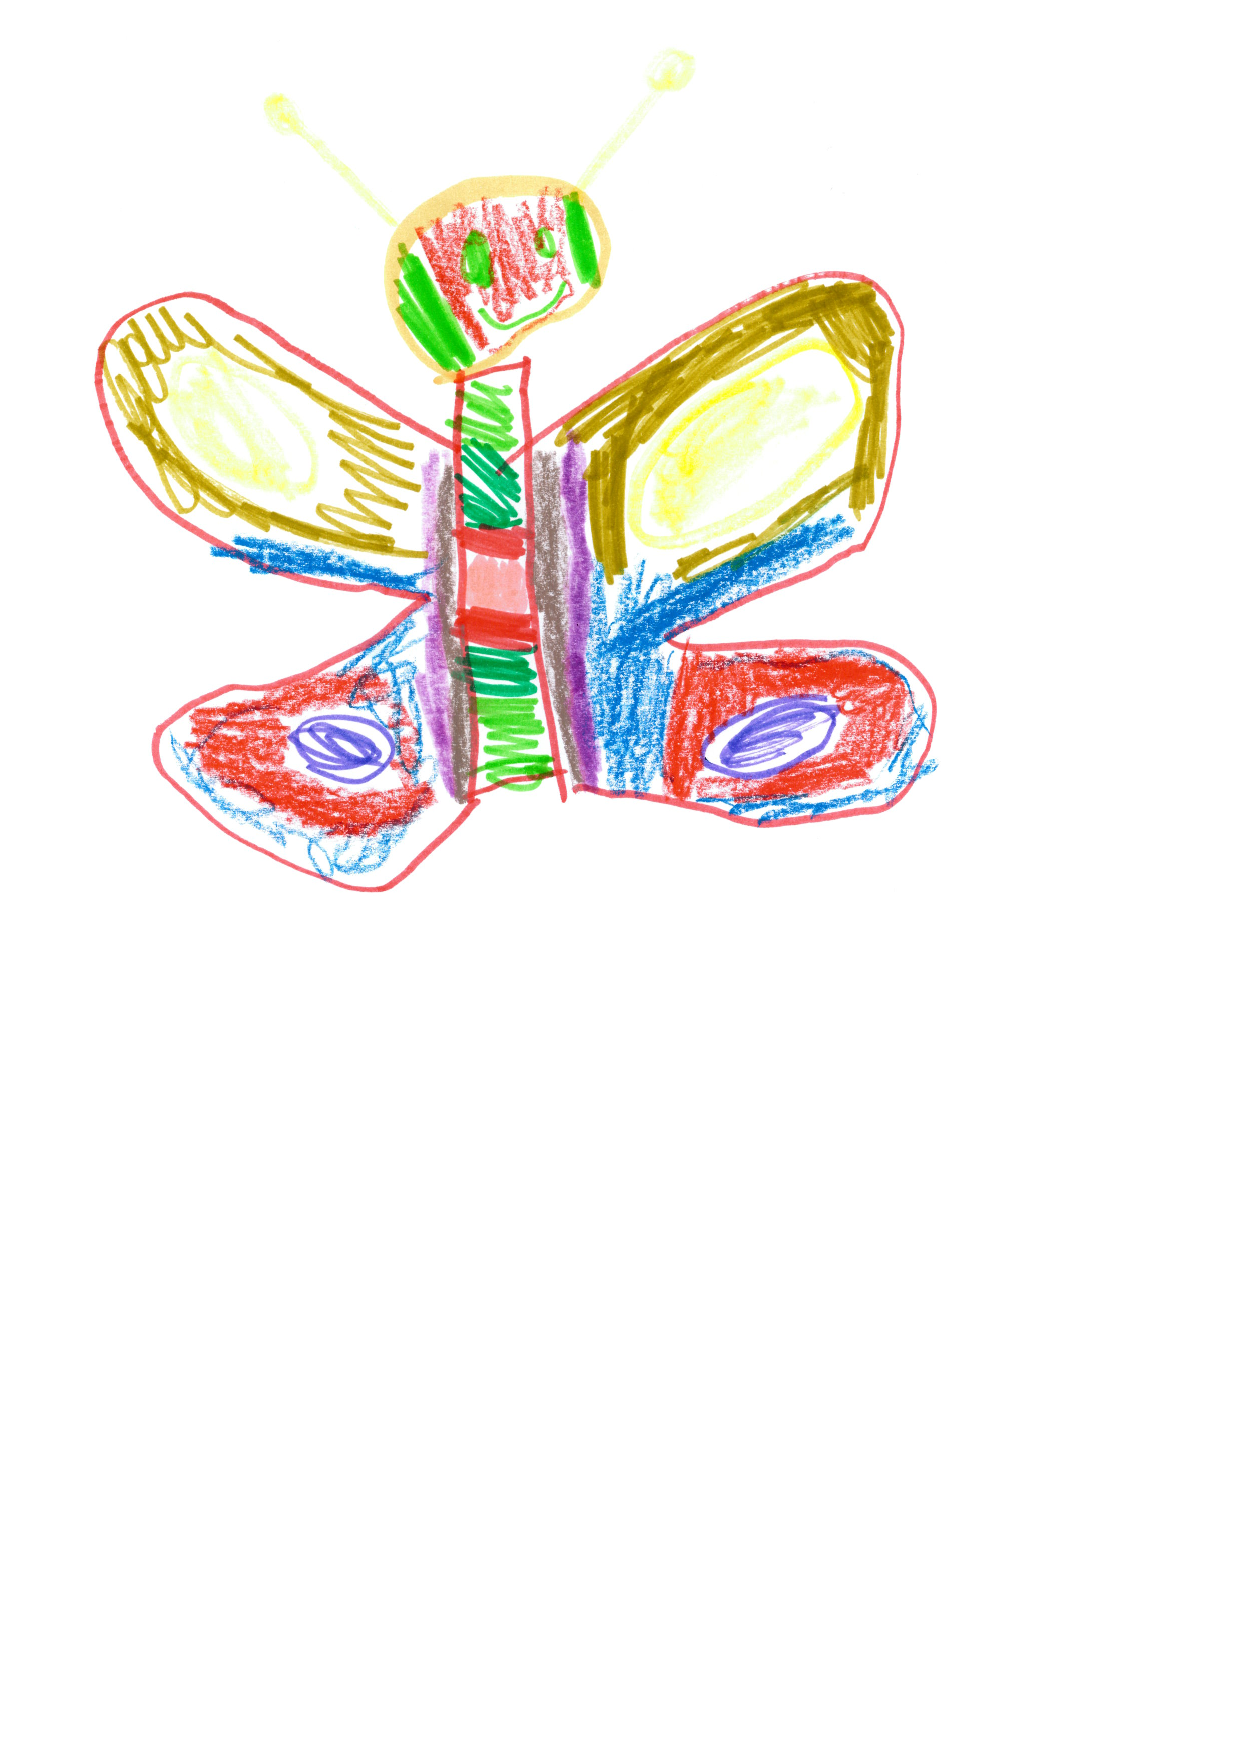
\includegraphics[scale=0.5]{pinarella.pdf}
\end{figure}

\chapter*{\FontH{\Huge Der weisse Adler}}
\addcontentsline{toc}{chapter}{Der weisse Adler}
\lettrine[lines=3]{\color{red}J}{a}, Johann war eitel. Ihr werdet sagen, dass das nicht schön ist, aber so ganz unrecht hatte er nicht. Schön war er schon, der Johann. Denn Johann war der einzige weisse Adler weit und breit. Die anderen waren braun oder grau, wie Adler eben so sind. Auch schön, aber nicht so speziell wie Johann und oft ist es ja gerade das Spezielle, was wir als besonders schön oder manchmal auch als besonders hässlich empfinden. Und die anderen Adler mussten zugeben, dass das besonders reine Weiss seiner Federn tatsächlich sehr schön war. Und so nahm es Johann niemand übel, dass er so eitel war. 

Johann tat das aber gar nicht gut. Er wurde beinah von Tag zu Tag ein bisschen eitler. 

\enquote{Ha, ihr seht ja alle so schmutzig aus, mit euren braunen Federn, als ob ihr gerade in den Dreck gefallen wärt.}, rief er den anderen zu. Aber auch das war schon bald unter seiner Würde. Mit nach oben geschobenem Schnabel zog er seine Kreise in der Luft. Erhaben fühlte er sich und auserwählt vom Schicksal. Mit Verachtung blickte er auf die anderen Adler herab. Es dauerte nicht lange, da redete er sich sogar ein, der König der Adler zu sein. Und so benahm er sich auch.

Eigenartig war, dass die anderen Adler ihm glaubten. Sie dachten, weil Johann so Einzigartig aussah, müsse er wohl auch etwas besonderes sein. Und wer so besonders ist, ist sicher dazu bestimmt, der König zu sein. Also brachten sie ihm Mäuse, wenn er Hunger hatte und erfüllten ihm auch sonst alle Wünsche. Ein paar wenige Adler, die ihm besonders viele Mäuse brachten, standen in der Gunst von Johann weit oben. Sie bekam zur Belohnung von ihm eine weisse Feder geschenkt. Und weil Johann die nur selten verschenkte, waren diejenigen, die eine hatten, auch etwas besonderes und genossen bei den anderen Adlern hohes Ansehen. 

So ging es einige Jahr ganz gut. Johann war der König, er hatte seine treuen Freunde und konnte regieren wie er wollte. Nicht dass er das sehr ausgenutzt hätte. Eigentlich war er nur etwas faul und liess sich gerne bedienen. Hochnäsig zog er seine Kreise am Himmel.

Ein Adler-Sprichwort sagt, dass wer hoch steigt, auch tief fällt. Das habt ihr vielleicht schon einmal gehört, bei uns Menschen gibt es das ja auch. Und so erging es auch Johann. Eines Tages kam er auf die Idee, dass ein König auch einen Thron brauche. Aber was wäre denn gut genug, ein Thron für den König der Lüfte zu sein? Die Sonne war zu heiss. Der Mond war zwar schön, aber mal war er gross und rund und dann wurde er immer schmaler. Das passte Johann gar nicht und auch das blasse Gelb gefiel ihm nicht. Als einmal jemand vorgeschlagen hatte, er möge sich doch auf eine Wolke setzten, war er beleidigt.

\afterpage{
    \begin{figure}
        \thispagestyle{empty}
        \centering
        
\includegraphics[width=\textwidth]{bilder/adler.pdf}
    \end{figure}
    \clearpage
}


\enquote{Die Wolken sind für den gemeinen Adler, nicht aber für ihren König.} Und so blieb nur der Regenbogen übrig. Der war aber tatsächlich besonders gut geeignet! Die herrlich leuchtenden Farben passten wunderbar zu den weissen Federn unseres Johann. 

Zufrieden mit seiner Wahl beäugte Johann den Regenbogen von allen Seiten und beschloss, dass hier sein Thron sein soll. So lud er alle Adler und auch die anderen Vögel des Himmels ein, Zeugen seiner feierlichen Thronbesteigung zu werden. Niemand traute sich die Einladung abzulehnen, immerhin war Johann ja der König. Und so putzte sich alles, was fliegen kann heraus und versammelte sich um den Regenbogen.

Johann, zufrieden so viele Bewunderer zu haben, plusterte sich nochmals gewaltig auf, flog bis an den höchsten Punkt des Regenbogens und setzte sich.

\enquote{Auf den Regenbogen setzten?}, höre ich euch fragen. Da habt ihr Recht, natürlich geht das nicht. Ein Regenbogen besteht nur aus Licht und auf Licht kann man sich nicht setzen. Ihr wisst das, aber Johann wusste das nicht! Und so plumpste er direkt durch den Regenbogen durch. Alle Adler und alle Vögel fingen an zu lachen. Und das Schlimmste war, der Regebogen hatte das weisse Federkleid unseres Johann ganz verfärbt. Hier ein roter Streifen, dort violette Tupfer und dazu überall gelbe und grüne Sprengsel. So sehr Johann auch flatterte und zappelte, die Farbe wollte nicht abgehen. Ja, wieder war Johann etwas besonderes, aber nicht mehr von der schönen Sorte.

\enquote{Hahaha, da kommt ja unser Fasnachts-Johann!}, riefen die anderen Vögel, \enquote{Der sieht ja aus wie ein Clown.} Und dabei blieb es. Vorbei war die Zeit vom König Johann. Niemand brachte ihm mehr Mäuse wenn er Hunger hatte, niemand putzte sein Federkleid und bewundert wurde er auch von niemandem mehr. Seine einstigen Freunde vermieden es, mit ihm gesehen zu werden. Die weisse Feder, die er ihnen geschenkt hatte, versteckten sie im Wald. Keiner wollte erinnert werden, einmal so einen bunten Vogel bedient zu haben. 

Und es wurde sogar immer schlimmer für ihn. Schon riefen die ersten anderen Adler:

\enquote{Hey, Fastnachst-Johann, bring uns Mäuse, wir haben Hunger.}, und fingen an, auf ihn einzupicken. Da blieb Johann nichts anderes übrig, als jetzt für die anderen Adler Mäuse zu suchen. Ein elendes Leben hatte er. Alle kommandierten ihn jetzt herum, so wie er sie einst kommandiert hatte. Das war nicht länger auszuhalten, beschloss er. Er konnte auch einfach nicht mehr. Er hatte keine Kraft mehr und es wurden zu viele Demütigungen.

Und so machte er sich auf den Weg und flog davon. Nach Norden flog er, weil ihm gerade nichts anderes einfiel. Weiter flog er und immer weiter, bloss weg von den anderen Adlern, immer höher in den Norden, wo nur Schnee und Eis sind und keine anderen Adler mehr wohnen. So kam Johann in das Reich der Schneekönigin.

Als die unseren Johann sah, freute sie sich. Denn ihr müsst wissen, dass am Nordpol -- und gerade da war unser Johann -- alles weiss ist. Überall nur Schnee und Eis. Kein Baum, kein Strauch und schon gar keine Blume oder sonst etwas, dass nicht weiss ist. Und so freute sich die Schneekönigin sehr, als unser bunter Johann geflogen kam. 

\enquote{Gute Tag, Johann}, sagte sie. Und nach einem langen Blick: 

\enquote{Wie schön Du bist.} 

\enquote{Ach, wenn es nur wahr wäre.}, seufzte Johann und erklärte: 

\enquote{Es ist noch gar nicht lange her, da war ich der Schönste Adler unter der Sonne. Rein und weiss gerade so wie der Schnee hier. Sogar König bin ich gewesen, weil ich so rein war. Aber ich wurde überheblich und hab nicht Recht getan. Ich bin faul geworden und habe mich füttern lassen. Und dann wollte ich zum König aller Vögel werden und vom Regenbogen aus regieren. Da bin ich gefallen. Meine Federn haben sich verfärbt wie ein Hemd beim Waschen und alle haben mich verstossen. So bin ich zu dir gekommen.}

Die Schneekönig verstand, dass Johann aufrichtig bereut hat und es ihm Leid tat, so überheblich gewesen zu sein. Da küsste sie ihn auf die Stirn. Ganz zart und vorsichtig. Hätte sie ihn mehr geküsst, wäre Johann sofort erfroren, denn alles, was die Schneekönigin berührt, wird sofort zu Eis. 

Ein eiskalter Schauer erfasste Johann. Noch nie hatte er so gefroren. Seine Flügel wurden steif und er konnte sich kaum bewegen. Die Federn wurden hart, als wären sie aus Glas. Ein paar brachen nur schon durch den Wind. Aber auch die Reste des Regenbogens in seinen Federn gefroren. Und sobald er sich ein bisschen erholt hatte und sich etwas besser bewegen konnte, fielen sie klirrend auf den kalten Boden.

Johann war glücklich. Er verbeugte sich zum Dank tief vor der Schneekönigin, breitete die Flügel aus und flog wieder zurück in den Süden. Dort lebte er von nun an als Adler unter Adlern. Weiss zwar und anders als die anderen, aber weder besser noch schlechter als sie. \hfill {\color{red}\decofourleft}

\chapter*{\FontH{\Huge }}
\lettrine[lines=2]{\color{red}A}{ls} die grosse Krähe die Menschen erschuf, lebten diese in einem Dorf auf einer Insel mitten Meer. Alle Menschen waren glücklich. Das Meer wimmelte von Fischen, Obst und Gemüse wuchsen prächtig und ab und an liess sich auch ein Wildschwein fangen. Das waren dann immer besondere Tage. Die Menschen zogen ihre schönsten Kleider an und trafen sich auf dem Platz des einzigen Dorfes und machten Musik und sangen solange das Schwein über dem Feuer bruzelte.

Die Menschen achteten die grosse Krähe und brachten ihr jede Woche kleine Geschenke. Das waren meistens Muscheln, die die Kinder am Strand gefunden hatten oder der Zahn eines Wildschweins oder auch eine besonders schöne Blume. Dafür beschützte die Krähe die Menschen und zeigte ihnen, wie man das Feld bestellt und Häuser baut.

Die grosse Krähe lebte auf dem höchsten Berg der Insel auf dem höchsten Baum. Von dort konnte sie die ganze Insel überblicken. Wenn jemand Hilfe brauchte, kam sie geflogen und tröstete die Menschen. Wenn jemand krank wurde, setzte sie sich so lange neben das Krankenbett, bis der Kranke wieder gesund war. Die Menschen liebten die Krähe dafür wie ihre Mütter.

Karnouk war einer der Dorfbewohner. Er war jung und schön und wurde von allen geachtet. Er konnte schneller laufen als alle anderen und interessierte sich für alles was die Menschen damals kannten, was allerdings nicht sehr viel war. Am liebsten sass er am Strand und beobachtete die Vögel oder die Fische. Kanouk war der einzige, der wusste, wo sich die Wildschweine am Tag versteckt hielten, aber das verriet er niemanden, denn er dachte, dass die Wildschweine alleine entscheiden sollen, wann sie gefangen werden wollten.

Einmal brach sich ein alter Mann auf der Suche nach Beeren im Wald ein Bein, als er über eine Wurzel stolperte. Karnouk hörte die Hilferufe und kam herbeigeeilt. Auch die Grosse Krähe kam und sagte, dass Karnouk nun nach Hause gehen könne, sie werde bei dem Mann bleiben. Aber Karnouk hatte eine bessere Idee. Geschickt band er zwei starke Äste so zusammen, dass der alte mann sich darauf legen konnte und Karnouk zog ihn zurück ins Dorf. Dort konnte er von seiner Töchtern versorgt werden, die ihn pflegten, bis das Bein wieder gesund war.

Die grosse Krähe aber rief: 

\enquote{Ihr Menschen, ich habe Euch immer geholfen und war für Euch da. Ich habe Euch die Dinge gegeben, die ihr zum Leben braucht. Alles weitere ist Frevel und erzürnt mich.} Die Menschen wiegten die Köpfe hin her und versprachen, nichts mehr selbst erfinden zu wollen, auch wenn es sehr praktisch wäre. Nur Karnouk schwieg. Er dachte, dass es doch nicht falsch sein kann, den Menschen zu helfen. Aber wusste auch, dass er noch mehr woltle als nur den Menschen zu helfen, er wollte die Welt kennen lernen. Oft sass er am Strand und blickte in die Ferne. Ob es wohl noch mehr Inseln wie seine gäb? Vielleicht sogar noch andere Menschen?

So verging die Zeit, Karnouks Sehnsucht nach der Ferne wurde jeden Tag grösser, aber es war aussichtslos. Überall Meer und wenn er die anderen Dorfbewohner fragte, riefen die nur, er solle sie nur in Ruhe lassen, die Grosse Krähe werde wütend, wenn jemand so rede. Karnouk wollte das nicht glauben und machte sich auf, die grosse Krähe zu besuchen. Es dauerte einen Tag und eine Nacht bis auf den Berg der Krähe zu klettern.

\enquote{Ich weiss, warum Du kommst Karnouk.} sagte die Krähe. \enquote{Du willst hinaus in die Welt, aber ich warne Dich. Das ist gegen meinen Willen, Du sollst ausgestossen werden aus dem Dorf, wenn Du so weitermachst. Ausserdem höre meinen Rat: Dein Tun ist gefährlich. Von hier oben sehe ich die ganze Welt, aber ich sehe nirgends am Horizont auch nur das kleinste Zeichen von Land.} Enttäuscht kehrte Karnouk in sein Dorf zurück. Er hatte seinen Plan aufgegeben.

Wie jeden Herbst kamen auch in diesem Jahr die Stürme. Gewöhnlich waren die nicht sehr stark, nur hin und wieder wurden ein paar Palmenwedel weggeblasen, mit denen die Menschen ihre Dächer bedeckten. Dieser eine Sturm war etwas schlimmer und er hielt viel länger an als sonst. Der Wind wollte für fünf Tage und fünf Nächte nicht aufhören zu blasen. Die Menschen verliessen ihre Häuser und suchten Schutz in einer Höhle. Als der Sturm sich endlich wieder gelegt hatte, kehrten sie in ihr Dorf zurück und sahen, was der Wind angerichtet hatte. Viele Dächer waren abgedeckt, aber das war nicht schlimm, das konnte schnell repariert werden. Aber es war noch etwas anderes geschehen. Hier und da sassen kleine Tiere, wie sie die Menschen bis dahin noch nicht gesehen hatten. Und da sie sie vor allem auf den abgerissen Palmenwedeln fanden, nannten sie sie Heuschrecken. 

Alle waren sich einig, dass Heuschrecken hässlich waren. 

\enquote{Das ist kein gutes Zeichen} riefen sie, \enquote{Wir haben bestimmt die Grosse Krähe verärgert.} meinten sie. So überlegten alle, was sie wohl zu bedeuten hätten, aber da die Heuschrecken nach ein paar Tagen alle samt von den Vögeln gefressen wurden, gerieten sie bald in Vergessenheit. Nur Karnouk konnte sie nicht vergessen. Ihn quälte die Frage, wo die Heuschrecken wohl hergekommen waren. Hatte sie der Wind geboren? Das konnte er sich nicht vorstellen. Alle Tiere hatten Vater und Mutter, soweit er das beobachten konnte. 

Nachdem er sehr lange über die Frage nachgedacht hatte, rief er das Dorf zusammen und verkündete:

\enquote{Meine Freunde, ich habe lange darüber nachgedacht, wo die Heuschrecken wohl hergekommen sind. Ich glaube der Wind hat sie zu uns geweht, denn ihr wisst, sie waren erst nach dem schlimmen Sturm hier. Aber aus dem Wasser kommen sie nicht, denn sie sehen aus, wie unsere Käfer, sie müssen von einer anderen Insel sein.}

Da erhob sich grosses Gelächter bei den Menschen.

\enquote{Von einer anderen Insel?} riefen sie. \enquote{Schau dich doch um. Von unserem Berg aus sieht man das ganze Meer und weit und breit ist nur Wasser. Die grosse Krähe hat nur das Meer und unsere Insel erschaffen, dahinter kommt nichts mehr. Und jetzt lass uns in Ruhe mit deinen dummen Ideen. Du verägerst die Grosse Krähe und dann sind wir alle verloren.}

Karnouk konnte jetzt an nichts anderes mehr denken, als an die Frage, wie er wohl über das Wasser käme. Er war ein guter Schwimmer, gewiss, aber das Meer war viel zu gross. Da half ihm der Zufall. Als er eines Nachmittags am Strand sass, viel gerade vor ihm eine Kokusnuss ins Wasser und trieb mit den Wellen davon. Das war die Lösung. Er musste nur etwas bauen, dass wie eine Kokusnuss ist, aber gross genug, dass er darin Platz hatte!

Kanouk fing an vieles auszuprobieren, die Leute wunderten sich immer mehr und wurden imemr wütender auf ihn. Die Angst vor der grossen Krähe war einfach zu gross. Aber Karnouk hatte keine Zeit sich um solche Sorgen zu kümmern. Er warf grosse Steine ins Wasser und bastelte riesige Schalen aus Palmenwedeln, die er auch ins Wasser setzte, bis sie untergingen. Eines Tages rannte er durch das Dorf und rief schreiend 

\enquote{Ich hab's, ich hab's!}

Verwundert lief das Dorf zu der Stelle am Strand, wo Kanouk in letzter Zeit gesessen und gebastelt hatte. Etwas, dass ein wenig aussah wie eine Schüssel lag mit der Öffnung nach oben im Sand. Sie war aus dem Holz der Palmen gemacht und mit dem Harz der Nadelbäume gestrichen. 

\enquote{Was soll das denn sein?} fragten sie sich und kratzen sich am Kopf. \enquote{Ich nenne es Boot,} sagte Kanouk \enquote{Und ich werde damit über das Meer reisen!}. Da wurden die Dorfbewohner zum ersten Mal richtig neugierig. Es stimmte ja, was Karnouk gesagt hatte. Irgendwo mussten die Heuschrecken hergekommen sein. Da kam die Grosse Krähe geflogen und rief mit donnernder Stimme:

\enquote{Ihr Menschen, ich hatte Euch gewarnt. Ihr sollt nicht Dinge bauen, die ich Euch nicht gezeigt habe. Ich weiss, dass Karnouk dieses Ding alleine gemacht hat. Deswegen will ich nur ihn bestrafen. Karnouk, Du bist ausgeschlossen aus unserer Gemeinschaft und sollst nie wieder in unser Dorf zurückkehren. Und wenn jemand von Euch Menschen auf seiner Seite ist, soll er es jetzt sagen.}

Die Menschen erschraken, senkten die Köpfe und liefen ins Dorf zurück. Kanouk blieb alleine am Strand zurück. jetzt hatte er nichts mehr zu verlieren. Er nahm seine Angel und so viele Lebensmittel, wie er finden konnte, steckte alles in seine Schale und stiess sie hinaus ins Meer. Er sprang hinein und tatsächlich. Die Schale schwamm und er mit ihr. Noch nie im Leben war Kanouk so aufgeregt wie in diesem Augenblick. Die Strömung erfasste ihn und langsam trieb er vom Strand weg in die offene See. Wind wehte ihm durch die Haare. Die Palmen am Strand wurden aus der Ferne immer kleiner. Und so trieb Kanouk davon, um nie wieder auf seine Insel zurückzukehren.

Viele Tage lang sah Kanouk nur Wasser, so weit er blicken konnte. Er bekam Angst. Gegen den Hunger konnte er fischen, trinken konnte er das Wasser des Regens. Als er schon glaubte, nie wieder Land sehen zu werden sah Kanouk eine Möwe. Und da wusste er, dass erbald Land finden würde. So wurde Kanouk der erste Mensch, der das Festland erreichte.

Die Menschen in dem Dorf aber konnten Kanouk nicht vergessen. Was war wohl aus ihm geworden? Und wer half jetzt, wenn sich jemand verletzt hatte. Nur der Trost der Krähe machte niemanden gesund, dass merkten die Menschen jetzt. Und eines Tages vertrieben sie die Krähe und fingen an, gemeinsam eine grosse Schale zu bauen, damit sie hinaus fahren konnte aufs Meer, um Kanouk zu suchen.

\chapter*{\FontH{\Huge Das Gespenst Jonathan}}
\addcontentsline{toc}{chapter}{Das Gespenst Jonathan}

\begin{quote}Vor drei Wochen habe ich zum ersten Mal in meinem Leben ein Gespenst gesehen. Klar, ich habe mir natürlich hin und wieder vorgestellt, dass es welche gibt, aber das meine ich nicht. Ich habe auch schon einmal gedacht, dass ich eines sehe, aber das war dann doch nur die frisch gewaschene Jacke von Frau Maier, unserer Nachbarin, die der Wind von der Leine gerissen hatte. Hab ich mich damals erschrocken! Die kam mir nämlich direkt entgegengeflogen und zwar nachts! Ich bin vor Schreck vom Fahrrad gestürzt und habe mir dabei die Hose zerissen. War das eine Aufregung und Mama wollte mir erst gar nicht glauben. Aber das will ich hier gar nicht erzählen, die Geschichte vom richtigen Gespenst Jonathan ist viel interessanter.  Das es Jonathan heisst, habe ich erst später erfahren. Aber ich will Euch mal die Geschichte von Anfang an erzählen, ich komme erst in der Mitte dazu.
\end{quote}

\lettrine[lines=2]{\color{red}K}{rrrawum.} Mit einem lauten krachen fällt die Rüstung von Ritter Odo von Gladez um. Die weisse Frau von Burg Lauenstein kommt durch die Wand gleich hinter der Rüstung geflogen und sieht sich den Haufen alten Blechs auf dem Boden an.

\enquote{Jonathan!} ruft sie, \enquote{Komm sofort hierher!} Mit gesenktem kommt auch Jonathan. Jonathan ist der Sohn der Weissen Frau, die eigentlich Otilia Brigitta Walburg Peternella von Abendberg heisst. Aber alle nennen sie die weisse Frau und das schon seit vierhundert Jahren. Sie ist nämlich ein Gespenst und die Mama von Jonathan, der natürlich auch eines ist. 

\enquote{Was soll ich nur mit Dir machen?} seufzt die Mama. Andauernd wirft Jonathan etwas um. Er passt einfach nicht auf, wenn er zu schnell durch die Wände geflogen kommt und nicht merkt, dass in dem Raum zum Beispiel eine Vase oder Kleiderständer steht. Gespenster können nämlich nur durch Wände fliegen, durch andere Sachen nicht. Und Jonathan war eben ein besonders schreckhaftes Gespenst. Immer wenn er glaubt, dass Menschen in der Nähe sind, nimmt er Reissaus und saust durch Burg Lauenstein, um sich zu verstecken. Besonders vor Kindern hat er furchtbare Angst. Die sind immer laut und frech und ärgern sich gegenseitig. 

Burg Lauenstein müsst ihr wissen, ist eine alte Burg. Tagsüber kommen Besucher aus der Umgebung und sehen sich an, wie die Menschen früher so gewohnt haben. Und zu einer alten Burg gehören eben auch Gespenster, die man allerdings nie am tage sieht und auch Nachts nur, wenn man sehr viel Glück hat. Seitdem irgendjemand mal auf die Idee gekommen ist, zu behaupten, dass Gespenster ganz gefährlich sind, haben sie angefangen, sich in den Kellern und Türmen oder wenigstens den Truhen der alten Burgen und Schlösser zu verstecken. Die allermeisten haben sich aber in Büchern versteckt und leben jetzt nur als Geschichte weiter. Eigentlich kenne ich kein Gespenst mehr, dass nicht nur in Büchern lebt, die weisse Frau und ihr Sohn Jonathan sind vielleicht die letzten.




\mdfsetup{
%
frametitle={
%
\tikz[baseline=(current bounding box.east),
outer sep =0pt]
\node[anchor=east,rectangle,fill=red]
{\color{white} \small Nina \& Oma Lena};},
frametitleaboveskip=\dimexpr-\ht\strutbox\relax
}
\pagenumbering{gobble}
\pagestyle{empty}
\section*{\FontH{\Huge Der Fall der verschwundenen Schmetterlinge}}
\centerline{\Huge \color{red}\SixFlowerPetalDotted}
\vspace{13pt}
\centerline{\bf \large\color{red}Für Papapa zum Geburtstag }
\vspace{13pt}
\centerline{\bf \color{red} von Linda, Paula, Doris und Gordon}
\vspace{13pt}
\centerline{\huge \color{red}\SixFlowerPetalDotted}
\vspace{13pt}
\centerline{\LARGE \color{red}\SixFlowerPetalDotted}
\vspace{13pt}
\centerline{\Large \color{red}\SixFlowerPetalDotted}
\vspace{13pt}
\centerline{\large \color{red}\SixFlowerPetalDotted}
\vspace{13pt}
\centerline{\normalsize \color{red}\SixFlowerPetalDotted}
\vspace{13pt}
\centerline{\small \color{red}\SixFlowerPetalDotted}
\vspace{13pt}
\centerline{\footnotesize \color{red}\SixFlowerPetalDotted}
\vspace{13pt}
\centerline{\scriptsize \color{red}\SixFlowerPetalDotted}
\vspace{13pt}
\centerline{\tiny \color{red}\SixFlowerPetalDotted}

\newpage
\pagestyle{scrheadings}
\pagenumbering{arabic}

\lettrine[lines=3]{\color{red}D}{as} Mobiltelefon klingelt und weckt Fenja aus dem Schlaf. Es ist noch sehr früh am Morgen. Zuerst bemerkt Fenja, dass es noch gar nicht hell ist. Eine Frechheit, wer ruft sie so früh an? Am Klingelton erkennt sie sofort, dass es Kommissarin Bettina Andermatt sein muss. Die Melodie vom rosaroten Panther.

Sofort ist sie hellwach. Fenja geht zwar noch in die Schule, aber sie ist sehr intelligent und kann sehr gut beobachten. Ihr fällt alles auf. Und sie vergisst nie, wann etwas passiert ist, egal wie lang das schon zurück liegt. Ihre Mutter sagt, das hätte sie von Papapa geerbt, als ob immer alles irgendwoher geerbt werden müsste. Aber in dieses Mal hat sie wohl Recht. 

Der Polizei ist es egal, wo das Talent jetzt genau herkommt, weiss es aber sehr zu schätzen und bittet sie regelmässig bei besonders verzwickten Fällen, bei der Aufklärung zu helfen. Es scheint wieder einmal soweit zu sein.

\enquote{Ja, aha, ich verstehe.} Fenja schreibt alles, was die Kommissarin sagt, in ein kleines Notizbuch, dass immer auf ihrem Nachtschränkchen liegt. Im Papiliorama in Kerzers sind Schmetterlinge verschwunden. Seltene, besonders schöne Exemplare der Gattungen \emph{Morpho peleides}.

\enquote{Entschuldigen sie die Frage, Frau Kommissarin, aber könnte es sein, dass die Schmetterlinge einfach abgehauen sind? Ich selbst würde auch jede Gelegenheit nutzen, wenn ich so eingesperrt wäre.} Im Zimmer kann man hören, wie die Kommissarin am anderen Ende der Leitung lauter wird. Für vorlaute Spässe habe sie keinen Sinn, schon gar nicht um diese Uhrzeit, hört man sie fast brüllen. Sie erklärt, dass es auffällig ist, dass nur Schmetterlinge eben jener Sorte verschwunden sind. Ausserdem sind auch alle Raupen weg.

Fenja verspricht der Sache sofort am nächsten Morgen nachzugehen und legt auf. Zunächst müssen die organisatorischen Dinge geklärt werden. Das Papiliorama liegt in Kerzers, das weiss Fenja aber schon. Erst neulich ist sie mit den Grosseltern dort gewesen. Das ist ein schöner Ausflug gewesen. Der erste Zug geht 7:32\,Uhr. Jetzt ist es 4:35\,Uhr. Genügend Zeit, sich vorzubereiten. Folgende Dinge kann Fenja mit Hilfe des Internet bereits recherchieren:

\begin{description}
	\item[Morpho peleides] \sffamily{Deutsch: Blauer Morphofalter. Der Schmetterling gehört zur Familie der Edelfalter. Die Flügel haben blaue Oberseiten und können eine Spannweite bis 12\,cm haben. Sie ernähren sich von faulenden Früchten.}
\end{description}

Fenja staunt. So riesige Schmetterlinge hat sie noch nie gesehen. Mit Hilfe des Lineals macht sie in ihrem Notitzheft ein Quadrat mit einer Höhe und Breite von je zwölf Zentimetern und zeichnet einen Schmetterling. Den malt sie blau aus. 

Dann beginnt sie ihren Rucksack zu packen. Sie benötigt:

\begin{enumerate}
  \item Die Detektivausrüstung bestehend aus ein paar sauberen Handschuhen, einer Lupe, einer Pinzette und ein paar leeren kleinen Tüten. Dazu ganz wichtig, gelbe Schnur vom Papapa.
  \item Orangensaft und Käsebrot. Aber ohne Tomaten, wie das Papa immer macht, da wird der Käse immer ganz weiss und das findet Fenja ekelig.
  \item Regenjacke, Mütze und Gummistiefel, erfahrungsgemäss finden Verbrecherjagden auch bei Schlechtwetter statt.
  \item Etwas Geld. Damit kann man dann so einiges kaufen, je nachdem, was gebraucht wird. Einmal war es nötig, sofort eine aufblasbare Kuh zu kaufen. Ein sehr merkwürdiger Fall war das damals.
  \item Einen Fotoapparat, um Tatorte dokumentieren zu können. Ein furchtbares Gerät. Es hatte lange gedauert, bis sie gemerkt hatte, dass man beim Bilderbetrachten drücken muss und nicht drehen darf. Grosi hatte es ihr dann gezeigt.
\end{enumerate}

Das alles passt wunderbar in ihren Rucksack. Noch die Schuhe und dann\dots steht plötzlich Carla vor ihr, das ist ihre kleine Schwester. Die wacht immer sehr früh auf und scheint etwas bemerkt zu haben. Carla ist zwar noch ziemlich klein, aber auch nicht dumm. Sofort begreift sie, dass Fenja etwas vor hat. Und sie weiss genau, dass es mit ihrer grossen Schwester immer aufregende Dinge zu erleben gibt.

\enquote{Wenn Du mich nicht verrätst, was du vor hast, fange ich so laut an zu weinen, dass Mama und Papa aufstehen.}

Das hätte gerade noch gefehlt. Die wollen nämlich eigentlich nicht, dass Fenja der Polizei hilft. Viel zu gefährlich meinen sie. Lächerlich. 

\enquote{Was willst du?} fragt Fenja. \enquote{Wenn Du leise bist, erlaube ich Dir so viele Trickfilme auf meinem Computer zu sehen, wie du willst.} Das ist zwar tatsächlich das verführerischste Angebot, dass die grosse Schwester machen kann, aber Carla lässt sich nicht beirren. Fenja seufzt. Ihr bleibt nichts anderes übrig, als Carla alles zu erklären und nach einer kurzen, aber überzeugenden Diskussion auch mitzunehmen. 

Aber das ist gar nicht so schlimm, überlegt Fenja. Eine kleine Schwester ist die beste Tarnung.   Jetzt in den Ferien sind viele Kinder im Papiliorama, da fallen sie beide gar nicht auf und können sich in Ruhe umsehen.

\begin{center}
\aldineleft
\end{center}
%\vspace{10pt}
% \centerline{\Huge \Dolphin[red]}
%\vspace{10pt}

Der Zug erreicht Kerzers pünktlich. Auf dem Weg zum Papiliorama schärft Fenja ihrer Schwester ein, dass sie nicht zum Spass hier sind. Die Schmetterlinge kann man sich auch ein anderes Mal wieder ansehen. Jetzt heisst es ermitteln und Spuren sammeln.

Der Direktor des Papilioramas, Herr Butterblom, weiss, dass Fenja kommen wird. Kommissarin Andermatt hat ihn schon informiert. Fenja entscheidet, dass es das beste ist, sich erst einmal in Ruhe umzusehen, um einen Eindruck vom Tatort zu bekommen. Die beiden Schwestern wollen getrennt ins Papiliorama gehen und sich in einer Stunde in der Cafeteria bei den Süssigkeiten treffen. Niemand wird glauben, dass Carla auch ermittelt.

Fenja hat sich überlegt, dass es sich bei den Dieben der Schmetterlinge nur Menschen handeln kann, die sich auf irgendeine Art für Schmetterlinge interessieren. Denn wertvoll sind sie nicht.  

\enquote{Herr Butterblom, wer könnte ein Interesse an diesen Schmetterlingen haben?} Fenja weiss, welche Fragen als erstes gestellt werden müssen. Herr Butterblom überlegt.

\enquote{Das weiss ich auch nicht. Es gibt natürlich Leute, die sich für Schmetterlinge interessieren und die selber züchten. Und da kommt es schon einmal vor, dass die hier ein paar Raupen klauen. Aber gleich alle? So etwas ist noch nie passiert.} 

\enquote{Kennen sie diese Sammler? Können sie mir vielleicht die Liste aller Namen geben?} will Fenja wissen.

\enquote{Natürlich nicht.} antwortet Herr Butterblom. Was für eine Frage. Jetzt kommen ihm doch Zweifel, ob es geschickt von Kommissarin Andermatt war, ein Kind zu schicken. Woher soll er denn die Namen der Leute kennen, die Schmetterlinge züchten? Aber Fenja ist etwas schlauer als er.

\enquote{Auf ihrer Web-Seite habe ich gesehen, dass sie auch Tagungen zu Schmetterlingen organisieren. Beispielsweise hat gerade letzte Woche jemand von der Universität einen Vortrag zu Schmetterlingen in den Alpen gehalten.} Fenja ist wirklich sehr gut vorbereitet. 

\enquote{Ich denke, dass alle, die sich für Schmetterlinge interessieren, auch an solchen Veranstaltungen teilnehmen. Es wäre sehr hilfreich, wenn sie mir die Anmeldelisten der letzten beide Jahre per E-Mail schicken könnten.}

Herr Butterblom ist verblüfft. Tatsächlich. Wenn es Züchter gibt, dann kommen die auch hierher und bei Veranstaltungen muss man immer vorher seinen Namen nennen, damit man reservieren kann. 
\begin{center}
\aldineleft
\end{center}

Zur selben Zeit schlendert Carla durch die Gänge des Papilioramas. Es ist gerade eine Sonderausstellung zum Thema \emph{Schmetterlinge in der Kunst}. Künstlerinnen und Künstler aus der Umgebung wurden eingeladen, ihre Sicht auf Schmetterlingen zu zeigen. Jemand hat einen grossen Schmetterling aus Stahl geschweisst, das ist das auffälligste Ausstellungsstück. Daneben gibt es ein paar Bilder an der Wand und eine Designerin hat sogar Kleidungsstücke mit Schmetterlingen bedruckt. Carla fotografiert alles sorgfältig mit der Kamera von Fenja.

\enquote{Alles grosser Unfug! Ganz schreckliches Zeug.} hört Carla neben sich sagen. Eine gross gewachsene Frau mit einem sehr eigenartigen Hut blickt verächtlich auf die ausgestellten Dinge. Carla fragt:

\begin{figure}[hb]
\centering
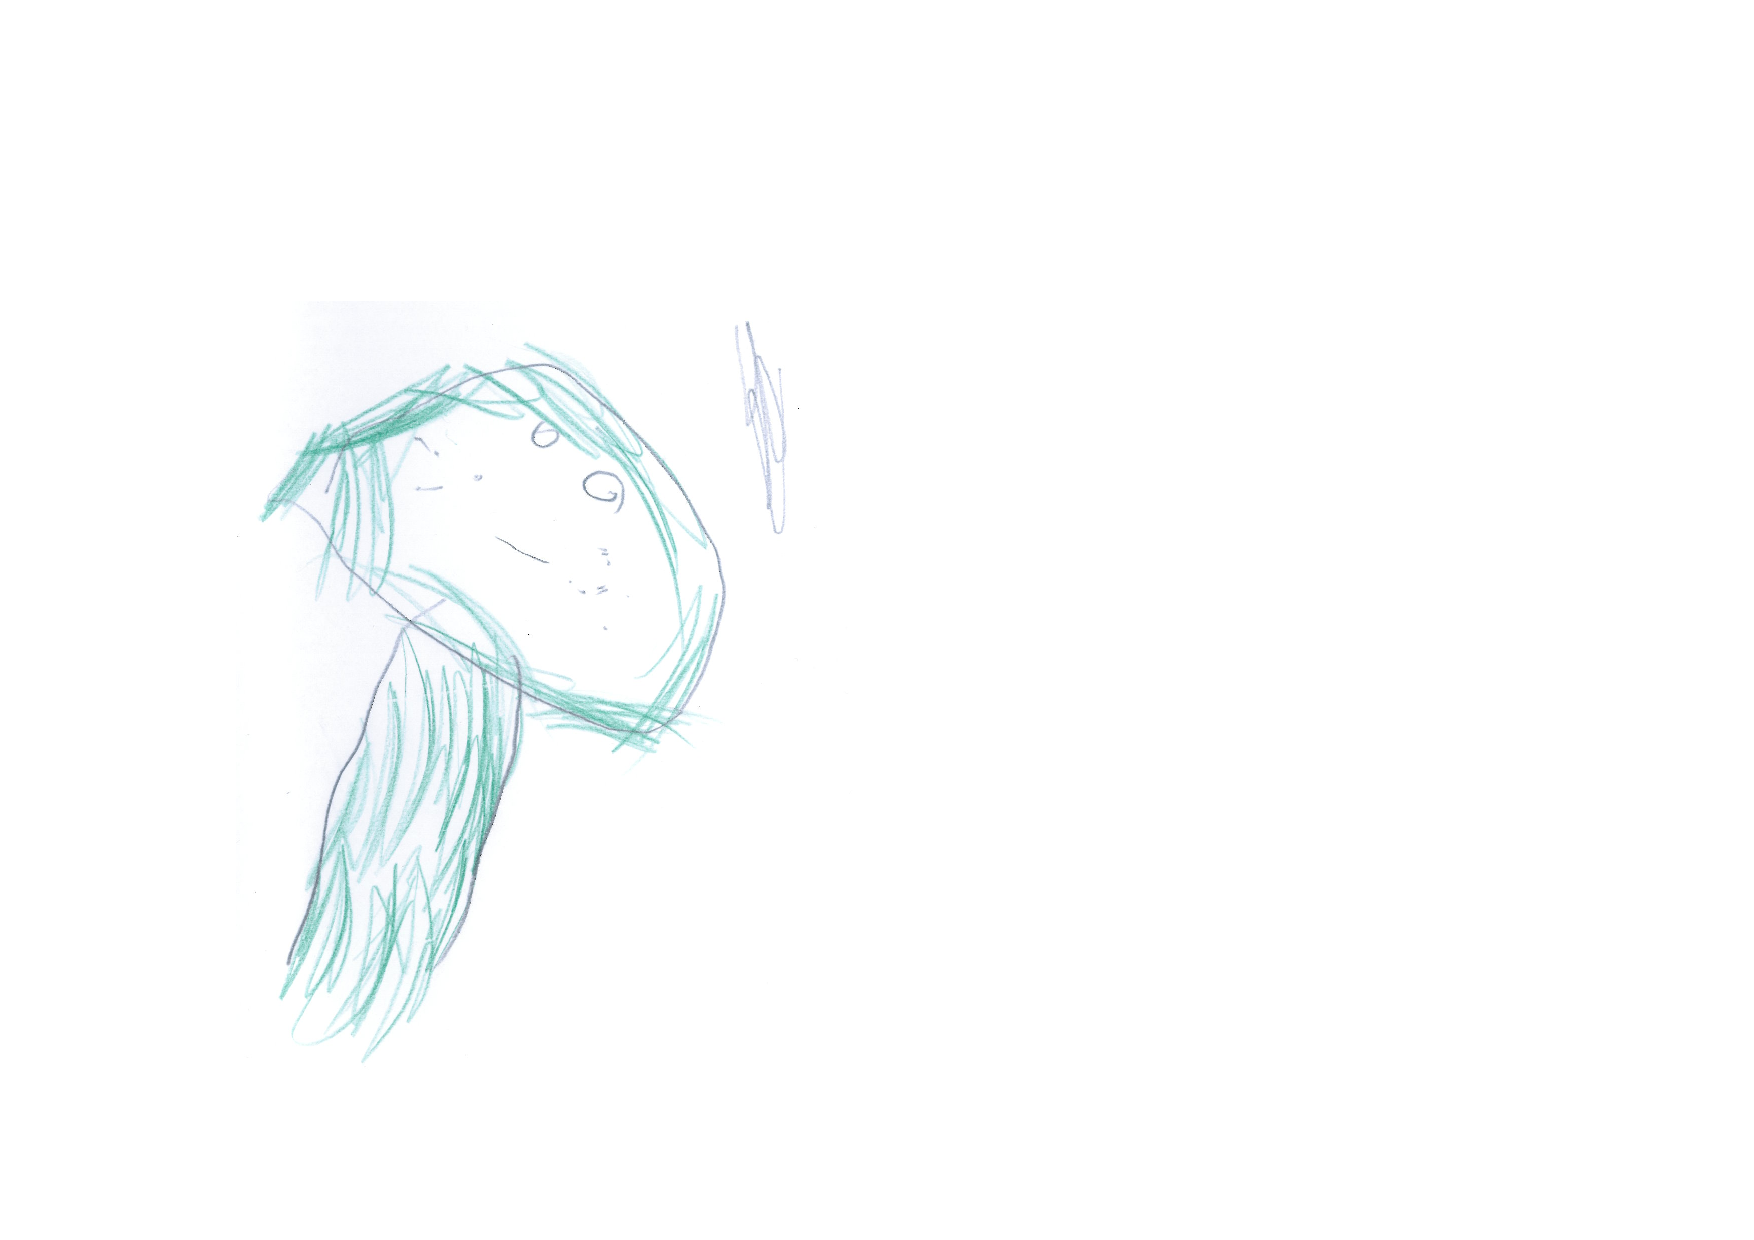
\includegraphics[width=.5\textwidth]{bilder/schmetterlingg.pdf}
\end{figure}

\enquote{Ihnen gefallen die Bilder wohl nicht besonders?}

\enquote{Natürlich nicht.} ruft die Frau mit sich überschlagender Stimme. \enquote{Das ist doch alles Unfug. Neben der Schönheit der Farben eines echten Schmetterlings, ist das hier alles blass und langweilig.} Und dann ergänzt sie:

\enquote{Darf ich mich übrigens vorstellen? Mein Name ist Verena Studer-Matt und das Kleid dahinten} dabei deutet sie auf die schmetterlingsgemusterten Kleider \enquote{sind übrigens von mir entworfen. Aber auch die finde ich mittlerweile ganz grauenvoll. Wer einmal die Schönheit eines Blauen Morphos gesehen hat, ist für derartiges verloren.} 

%\begin{figure}[h]
%\centering
%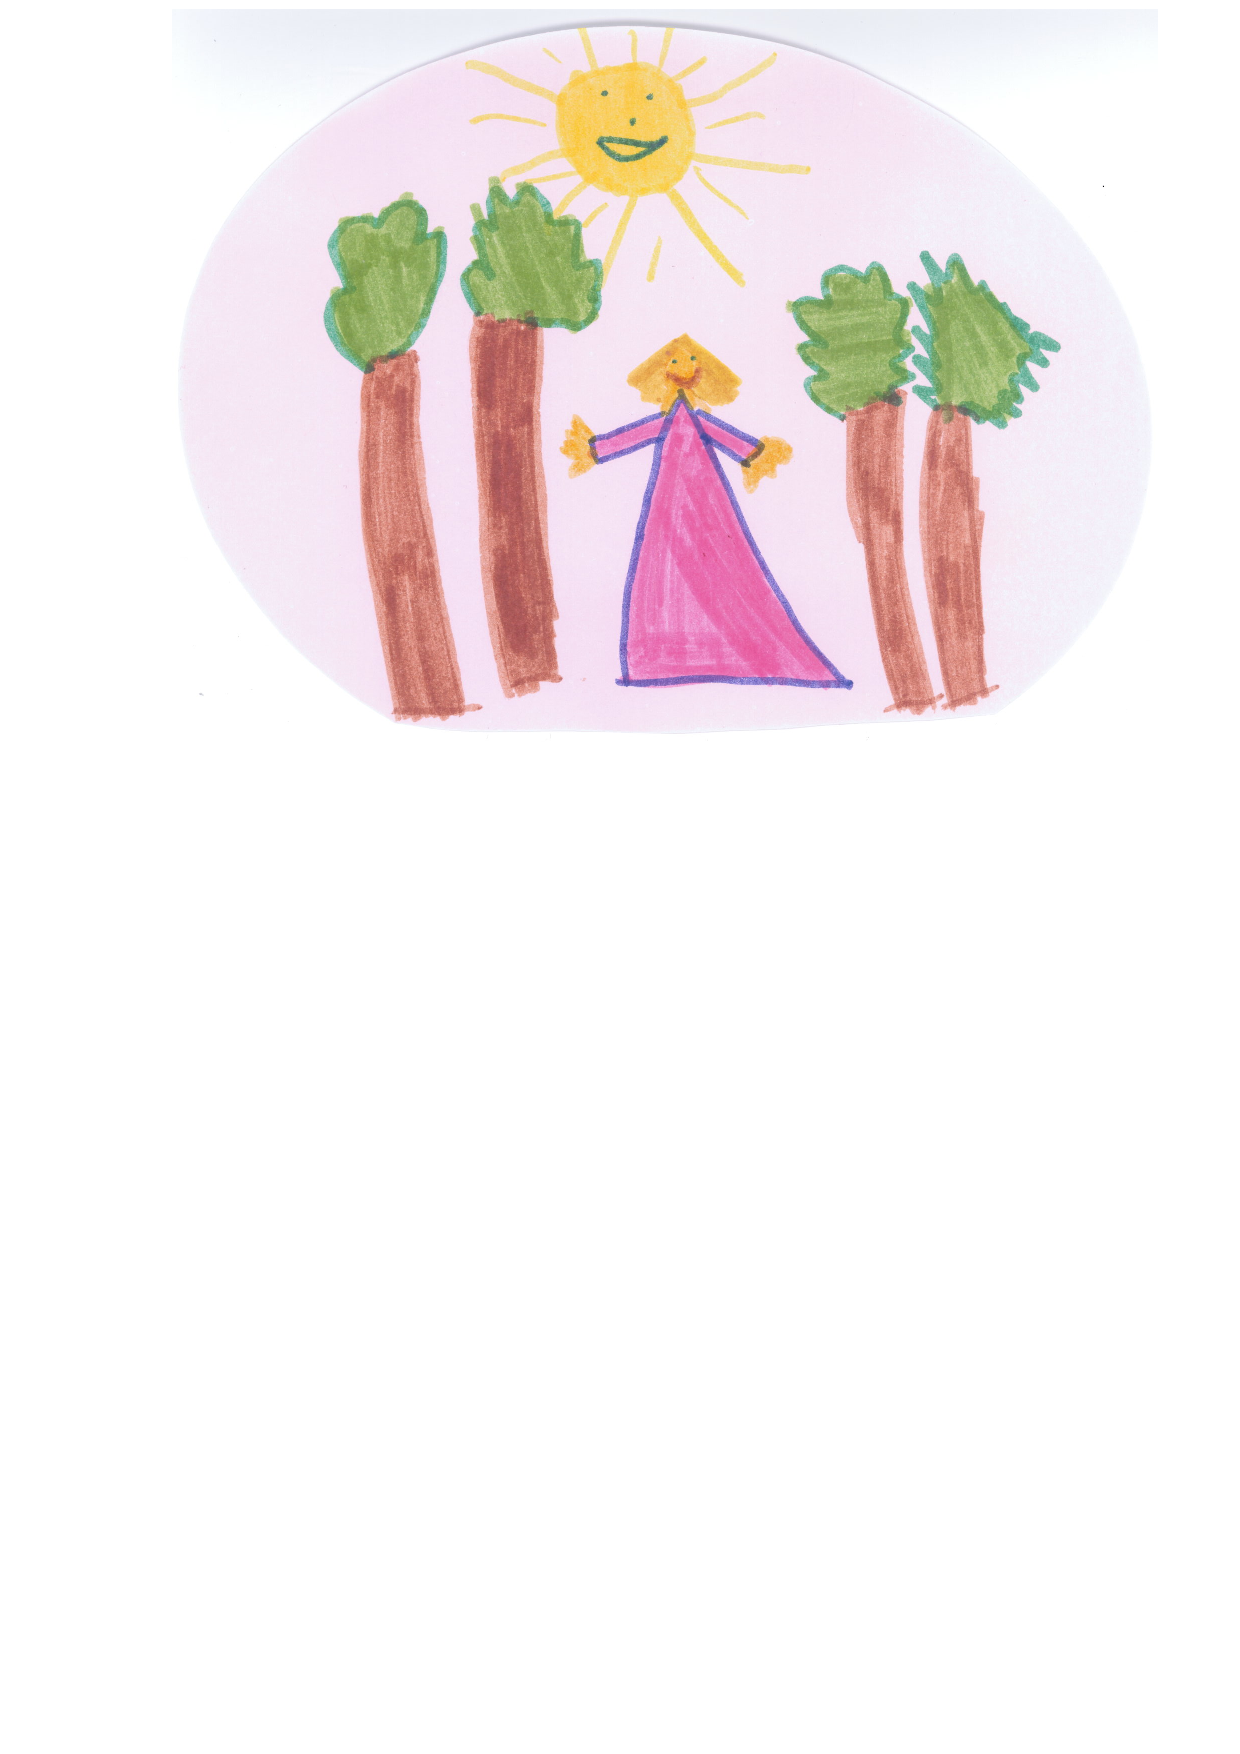
\includegraphics[width=.7\textwidth]{bilder/kerzers.pdf}
%\end{figure}

Mit einer Miene, die tiefen Ekel ausdrücken soll und ohne eine Antwort von Carla zu erwarten stapft die Dame davon. Ob sie weiss, dass gerade diese Schmetterlinge alle verschwunden sind, überlegt Carla?

Die beiden Schwestern treffen sich wie verabredet in der Cafeteria. Wie immer darf sich Carla nichts kaufen sondern muss das essen, was Fenja mitgebracht hat. Fenja erzählt kauend, dass man als nächstes bei den Sammlern und Züchtern nachfragen muss. Es sind im Moment die einzigen Verdächtigen. Und weil klar ist, dass sie hier nicht weiterkommen, beschliessen sie nach Bern zu fahren, an der Universität gibt es einen Spezialisten für Schmetterlinge. Das ist der, der neulich hier den Vortrag gehalten hat, am besten man fängt bei dem gleich an. Vielleicht hat der eine Ahnung, wer wohl ein Motiv hat, Schmetterlinge zu stehlen.
\begin{center}
\aldineleft
\end{center}

 Als sie in Bern ankommen, hat Fenja schon über das Internet herausgefunden, wie sie zur Universität kommen und wo sie dort den Schmetterlingsexperten finden. Dr.\,Adrìan Moreira heisst er, das Büro von ihm müssen sie jetzt suchen. \emph{Zoologisches Institut} steht über der Eingangstür. Als ob Fenja jeden Tag hier wäre, geht sie zielsicher zum Fahrstuhl und drückt den Knopf zum dritten Stock. Woher ihre Schwester wohl immer so genau weiss was zu tun ist, überlegt Carla.

\enquote{Hallo ich bin Adrìan} begrüsst sie ein junger Mann mit stark spanischem Akzent. Das verblüfft dann sogar Fenja. Sie hätte sich Professoren viel älter vorgestellt und das sagt sie ihm auch, um sicher zu gehen, dass sie mit dem richtigen spricht. Adrìan muss lachen. \enquote{Na erstens bin ich noch kein Professor und ausserdem seid ihr beiden ja auch nicht im typischen Alter von Detektivinnen.} Er schiebt den beiden je eine Dose Cola hin. Zu Hause dürfen sie die nie trinken, was aber jetzt natürlich keine der beiden stört. Nichts anmerken lassen, heisst es jetzt.

\enquote{Also, wie kann ich Euch helfen?} Fenja erklärt was passiert ist. Adrìan hört sehr aufmerksam zu.

\enquote{Nein. Da kann ich euch nicht helfen. Ich habe keine Ahnung, wer so etwas tun könnte. Aber halt, wartet einmal. Neulich war eine Dame hier, die hat sich genau für diesen Schmetterling interessiert. Und die wollte wissen, wie man es am besten schafft, dass die Flügel auch nach dem Tod der Schmetterlinge möglichst lange halten und ihr Blau behalten.}

\enquote{Wie heisst die Frau?} Fenja ist wie elektrisiert. Das ist die erste echte Spur. So etwas kann kein Zufall sein. Adrìan überlegt und schaut in seinem Computer nach.

\enquote{Ich befürchte, dass ich den nicht kenne. Ich glaube, die hat sich gar nie richtig vorgestellt. Aber ich kann sie euch beschreiben. Sie ist schon etwas älter, gross und wenn ihr mich fragt\dots} und statt etwas zu sagen tippt er sich mit dem Finger an die Stirn \enquote{Na jedenfalls hatte sie einen wirklich exzentrischen Hut auf. Riesig und mit Federn.} Jetzt ist Carla aufgeregt. 

\enquote{Die habe ich heute gesehen, im Papliliorama. Das ist die Frau, die die Kleider mit dem Schmetterlingsmuster gemacht hat!} Adrìan und Fenja sehen Carla verblüfft an. Carla erinnert sich, dass die Frau auch ihren Namen genannt hatte, aber den hat sie lengst vergessen. Namen kann sie sich einfach nicht merken. Und bevor Fenja böse ist, sagt sie lieber nicht, dass sie den Namen kennen sollte.

\enquote{Wie die heisst, weiss ich auch nicht, aber ich habe die Kleider fotografiert.} Adrìan und Carla blicken auf das Display des Fotoapparates. Fenja ruft derweil Herrn Butterblom an. Der weiss den Namen auch nicht auswendig, sieht aber schnell auf dem Schild unter dem ausgestellten Kleid nach. Studer-Matt heisst sie.

\enquote{Richtig}, ruft Carla, \enquote{jetzt fällt es mir auch wieder ein.} Fenja runzelt mit Blick auf ihre Schwester die Augenbrauen und schlägt aber ohne etwas zu sagen im Telefonbuch die Adresse nach. Mit kleinen Schwestern zu schimpfen lohnt sich nicht und den Namen haben sie ja jetzt auch so.

\enquote{Na ich komme mal besser mit.} sagt Adrìan.

Als sie bei Frau Studer-Matt ankommen, riecht es sehr verfault. Adrìan will an der Tür klingeln.

\enquote{Halt!} ruft Fenja. \enquote{Wenn die Schmetterlinge da drin sind, ist es besser wenn die Tür geschlossen bleibt. Die Schmetterlinge leben eigentlich in tropischen, also warmen Gebieten. Kalter Wind ist schädlich. Im Übrigen bin ich der Meinung, dass die Schmetterlinge sicher hier sind. Richt ihr nicht den Geruch? Das ist faulendes Obst, das Lieblingsessen des Blauen Morphofalters. Ich rufe jetzt Kommissarin Andermatt an, wir warten hier so lange.}

Adrìan ist verblüfft. Das hätte er eigentlich alles selber merken können. Hat er aber nicht. Zur Sicherheit bindet Fenja den Türknauf am Treppengeländer fest. So kann niemand von innen die Tür öffnen. Bei Verbrechern muss man vorsichtig sein! Eine Erfahrung, die Fenja schon häufiger gemacht hat. Genau wie immer ein paar Meter gelbe Schnur von Grossvater mit zu haben. Die war auch schon sehr oft nützlich. 

Eine halbe Stunde später ist die Kommisarin da. Sie hat auch gleich noch ein paar Kollegen mit gebracht, als Verstärkung. Sie klingeln jetzt doch an der Tür. Eine genervte Frau, die ganz offensichtlich tatsächlich Frau Studer-Matt ist, öffnet die Tür. Und auf ihrer Schulter sitzt auch schon der erste blaue Schmetterling.
\begin{center}
\aldineleft
\end{center}

Adrìan und Herr Butterblom fangen die Schmetterlinge in der Wohnung ein und bringen sie zurück ins Papiliorama. 

\enquote{Warum haben sie das getan?} Kommissarin Andermatt spricht die Frage aus, die alle brennend interessiert.

\enquote{Ich wollte, ich, \dots} Frau Studer-Matt kommt ins Stottern. Aber dann holt sie tief Luft und sagt: 

\enquote{Ich wollte das schönste und vollkommenste Kleid nähen, dass je ein Mensch getragen hat. Ich wollte es mit den Flügeln der Schmetterlinge besticken, den schönsten Pailletten der Welt. Das herrliche Blau dieser Schmetterlinge ist einfach unübertroffen. Das ist eine Erfindung, die so genial ist, dass vor mir noch niemand darauf gekommen ist. Ich werde vielleicht verhaftet, aber ich werde in die Modegeschichte eingehen. Das lasse ich mir auch nicht von euch Kleingeistern auch kaputt machen. Was sind schon ein paar Schmetterlinge gegen wahre Schönheit.}

Die Kommissarin schüttet den Kopf, Carla hat nicht ganz genau verstanden, was Frau Studer-Matt vor hatte und Fenja kann es sich nicht verkneifen zu erklären, dass schon früher Menschen in Süd- und Mittelamerika Kleider mit den Schalen von Käfern bestickt haben. Das ist nicht nur ganz ähnlich, sondern hält auch besser. 

Als die beiden Mädchen zu Hause ankommen, machen Mama und Papa geheimnisvolle Gesichter. 

\enquote{Na, habt ihr heute schön gespielt?} wollen sie wissen. Und noch während Fenja überlegt, ob man auch nicht schön spielen kann, zückt ihr Papa zwei Eintrittskarten hinter dem Rücken hervor.

\enquote{Überraschung: Morgen fahren wir alle zusammen nach Kerzers ins Papiliorama!} Da rufen die beiden Schwestern wie aus einem Mund:

\enquote{Oh nein, bloss nicht!} \hfill {\color{red}\decofourleft}


\chapter*{\FontH{\Huge Aus dem Leben des Karl Rebosam}}
\addcontentsline{toc}{chapter}{Aus dem Leben des Karl Rebosam}
Karl ist auch in den Grundfragen der Pädagigik unorthodox. Je nach Vergehen des Zöglings schlägt sich Karl selbst ins Gesicht. Blut ist ein \emph{must}. Das soll dem Knaben eine Lehre sein!

Gelegentlich ertappt sich Karl bei dem Gedanken, sein Kind zur Adoption frei zu geben.
\begin{center}
{\huge \textthing}
\end{center}
Karl ist heute sehr nachdenklich. Er hatte folgenden Algorithmus angewendet:
\begin{enumerate}
	\item Öffne das Telefonbuch.
	\item Bilde die Quersumme der Telefonnummer des ersten Eintrags beim Buchstaben \emph{A}.
	\item Notiere das Ergebnis und verfahre so bei allen weiteren Buchstaben.
	\item Addiere alle Ergebnisse und bilde die Quersumme.
	\item Bilde aus diesem Wert so lange die Quersumme, bis diese einstellig ist.
	\item Wiederhole alle vorhergehenden Schritte für den jeweils letzten Eintrag eines Buchstabens.
\end{enumerate}
Das Ergebnis erwies sich in beiden Fällen als $5$. Was hat das zu bedeuten? Voll innerlicher Welkeheit schritt Karl seine Sammlung ausgestopfter Nagetiere ab und empfand es einmal mehr als schmerzlich, dass ausgerechnet eine Ratte noch nicht zu integrieren gewesen war.
\begin{center}
{\huge \textthing}
\end{center}
An jedem achten Tag nach Neumond empfand Karl Rebosam Lust. Schon der Anblick der morgentlichen Zahnpasta, wie sie sich schlangenfraugleich aus der Tube auf seine Bürste windet und er diese dann in seinen Mund schiebt und nach einem kurzen Augenblick des Innhaltens sanft aber kräftig mit der Zunge zerdrückt, liess heissen Schweiss aus seiner Stirn triefen. 

Und wenn dann der  Toaster durch die Behandlung mit feuriger Glut aus zwei bleichen schwammigen Fladen, braune knusprige Wesen erschafft und diese mit einem Knall aus seinem inneren heraus spuckt, ist Karl der Ohnmacht jeweils schon recht nahe.
\begin{center}
{\huge \textthing}
\end{center}
Es stellte sich als kapitalen Fehler heraus, das falsch gegebene Rückgeld zu reklamieren. Die Bäckersfrau war nicht bereit, Kritik zu akzeptieren. Diese kategorische Charaktereigenschaft, gepaart mit einer Meisterschaft in der Schwitzkastentechnik, führten zu einer für Karl nicht vorhersehbaren Reaktion.

Karl verbrachte einen wesentlichen Teil des Vormittags unter der Achselhöle der sonst frommen Bäckersfrau. Er musste mit Respekt beobachten, wie die Bedienung der ihm nachfolgenden Kundschaft ganz reibungslos durch die Vermittlung nur eines Arms funktionierte. Im Grunde klappe sie sogar besser als mir beiden Armen, denn da Katls Gesicht beim Bezahlen jeweils tief in die Kasse gedrückt wurde, konnte er bei der Herausgabe des Wechselgeldes mitzählen. Ein weiterer Fehler war dabei der Bäckersfrau nicht vorzuwerfen. Ärgerlich war im Weiteren nur, dass er seine Pfeife nicht mitgenommen hatte.
\begin{center}
{\huge \textthing}
\end{center}
Heute hat Karl folgende annonce im Lokalblatt publizieren lassen: {\it Hundesalon Rebosam sucht per sofort einen Hundecoiffeur. Neben viel Libe zu den Vierbeinern erwarten wir einen männlichen Berwerber, der aus Gründen der Authenzität möglichst selbst stark behaart ist. Ausnahmen gelten nur für Träger eines Menjou oder eines Dali-Bärtchens. Weitere Auskunft erhalten sie unter Tel. \ldots. }

Natürlich gibt es diesen Hundesalon Rebosam gar nicht. Die Telefonnummer ist aber tatsächlich die unseres Karln.
\begin{center}
{\huge \textthing}
\end{center}
\hfill {\color{red}\decofourleft}


%Inhaltsverzeichnis
\newpage
\tableofcontents

\end{document}



